En esta sección, vamos a realizar experimentos para comprobar empíricamente tanto el tiempo de ejecución como la calidad de las soluciones devueltas por nuestro algoritmo goloso.

Como ya sabemos, el algoritmo de Dijkstra devuelve el camino de un nodo inical hacia todos. Particualarmente, a nosotros nos interesa el camino de $u$ a $v$. Por esto, se nos ocurrió una simple optimización: cortar la ejecución del algoritmo cuando alcanza $v$.

\begin{figure}[H]
  \begin{minipage}{0.5\linewidth}
    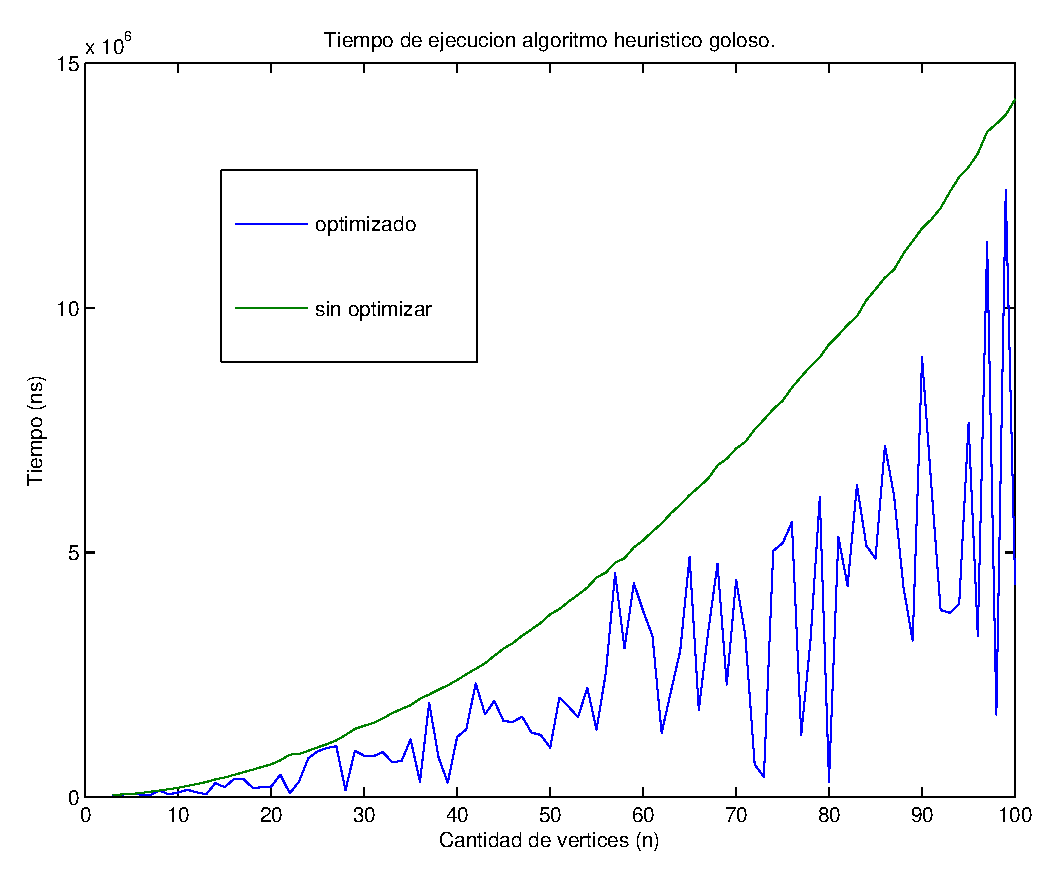
\includegraphics[width=\linewidth]{graficos/goloso_tiempo.eps}
    \caption{Tiempo ejecución goloso}\label{fig:goloso-tiempo}
  \end{minipage}
  \hfill
  \begin{minipage}{0.5\linewidth}
    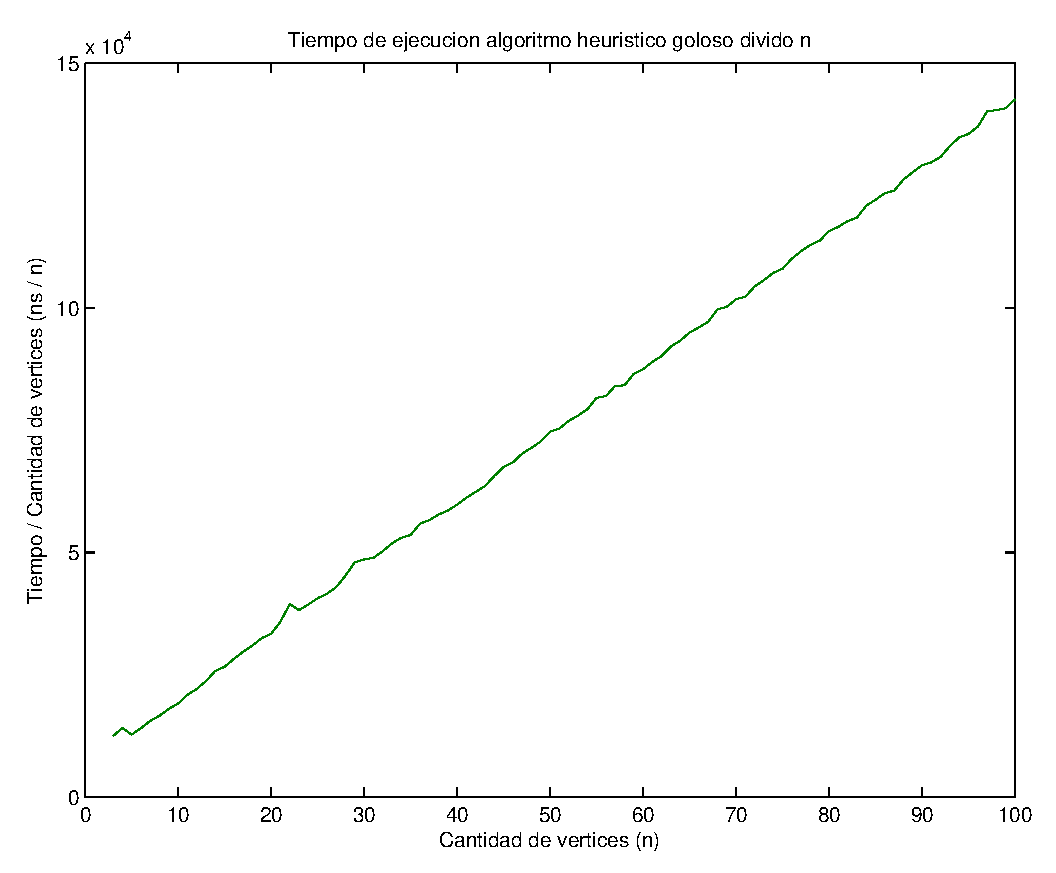
\includegraphics[width=\linewidth]{graficos/goloso_tiempo_div_n.eps}
    \caption{Goloso sin optimización}\label{fig:goloso-tiempo-n}
  \end{minipage}
\end{figure}

Como se puede observar en la figura \ref{fig:goloso-tiempo}, nuestro algoritmo sin la optimización se comporta de forma cuadrática. Esto es lógico ya que nuestro algoritmo sin la optimización corre el algoritmo de Dijkstra de principio a fin, utilizando listas de adyacencia.

Además, en la figura \ref{fig:goloso-tiempo} podemos observar que el algoritmo con la optimización tiene un tiempo de ejecución menor o igual al algoritmo sin la optimización. Esto depende del momento en que el algoritmo encuentra a $v$, con lo cual puede ser el primer nodo o el último según la corrida.

Luego, nos propusimos comparar la calidad de las soluciones entre el goloso y el exacto, para casos random. Cabe aclarar que vamos a utilizar casos con $n$ chico, ya que el algoritmo exacto tiene tiempo de ejecución exponencial.

%TODO estos graficos no son los correctos!

% \begin{figure}[H]
%   \begin{minipage}{0.5\linewidth}
%     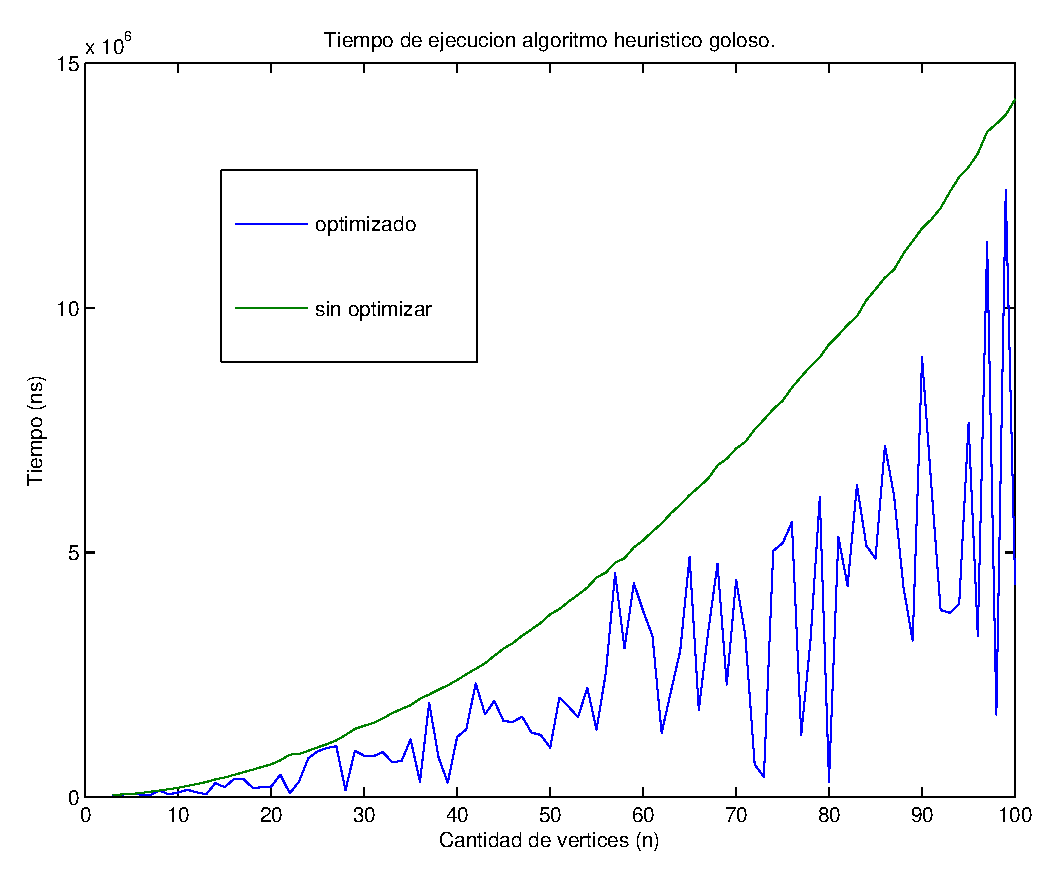
\includegraphics[width=\linewidth]{graficos/goloso_tiempo.eps}
%     \caption{Tiempo ejecución goloso}\label{fig:goloso-exacto-random}
%   \end{minipage}
%   \hfill
%   \begin{minipage}{0.5\linewidth}
%     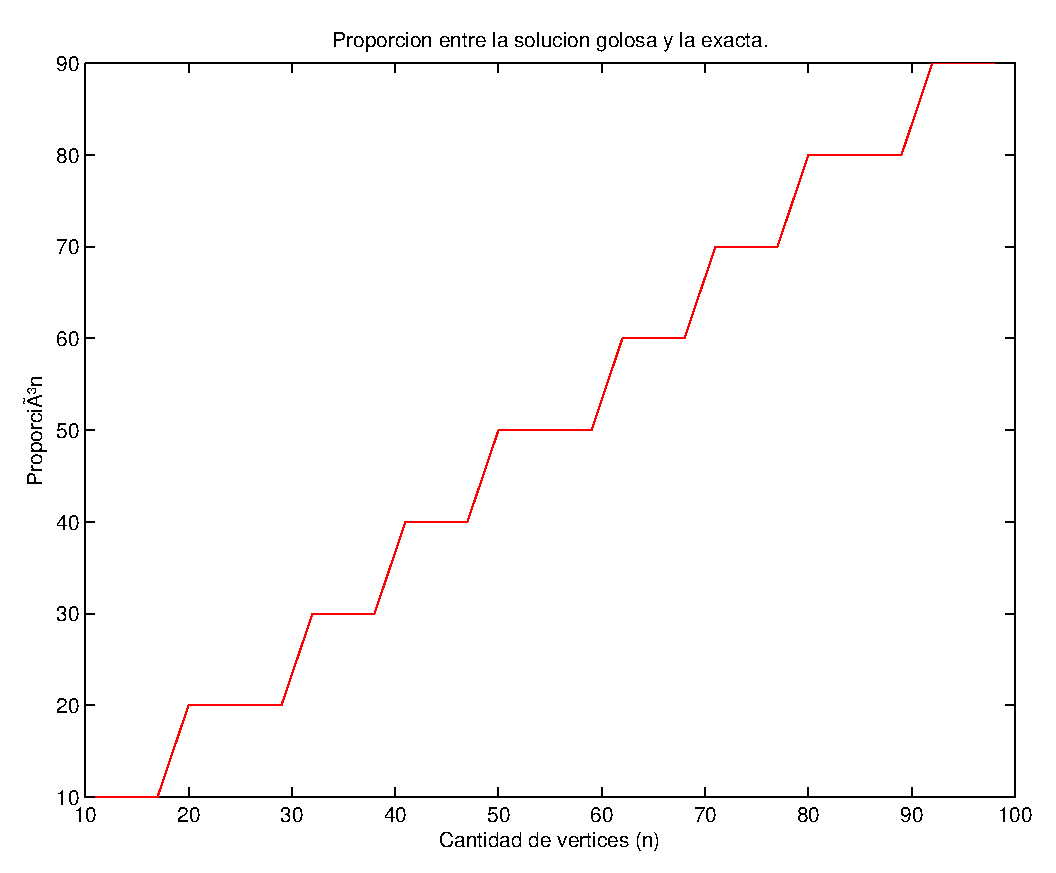
\includegraphics[width=\linewidth]{graficos/goloso_proporcion2.eps}
%     \caption{Tiempo ejecución goloso sobre n}\label{fig:estelousamos}
%   \end{minipage}
% \end{figure}

En los siguientes gráficos, vamos a comparar empíricamente la proporción entre los pesos $\omega_2$ totales de los caminos solución corriendo el algoritmo exacto y el goloso para la familia de grafos previamente mencionada. Creamos una función la cual recibe un parámetro que es la diferencia deseada entre el goloso y el exacto.

Sea $S$ la solución devuelta por el algoritmo exacto, y $S'$ la solución devuelta por el algoritmo goloso, vamos a gráficar $\omega_2(S')$ / $\omega_2(S)$ para distintos $n$.

\begin{figure}[H]
  \begin{minipage}{0.5\linewidth}
    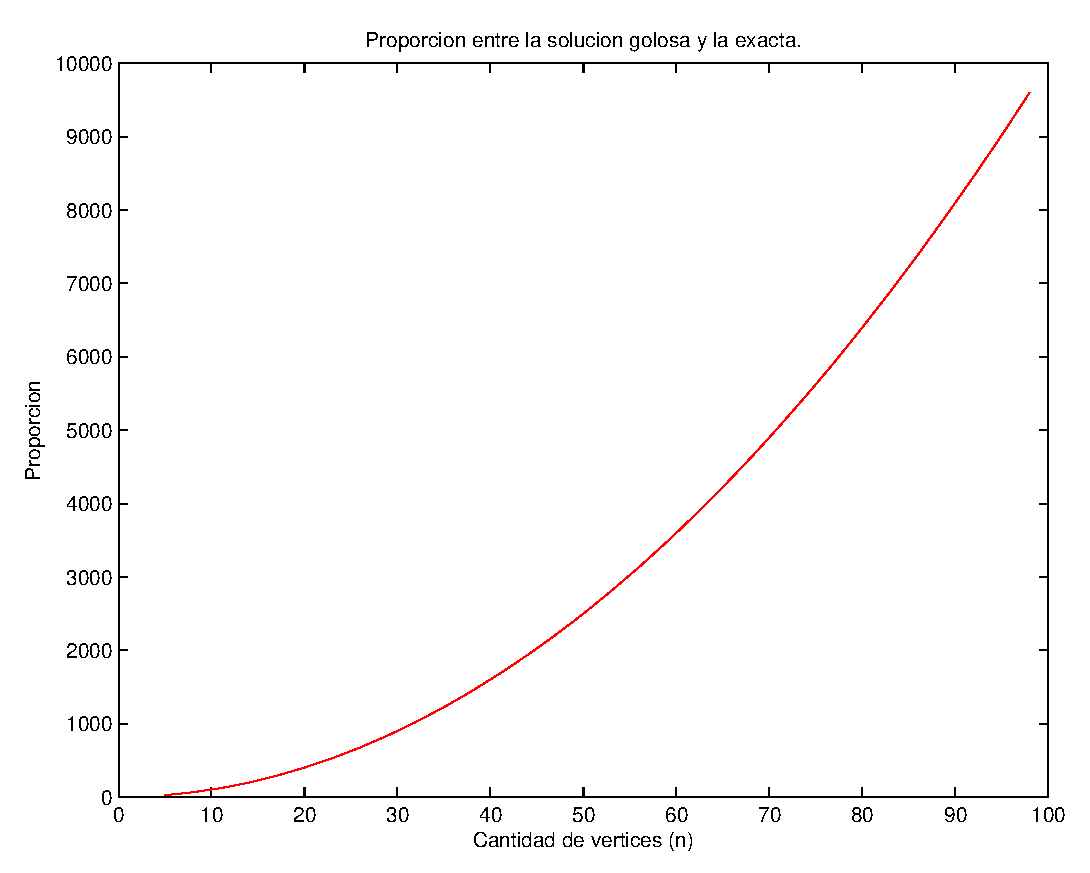
\includegraphics[width=\linewidth]{graficos/goloso_proporcion.eps}
    \caption{Comparación goloso exacto función $n^2$}\label{fig:goloso-n2}
  \end{minipage}
  \hfill
  \begin{minipage}{0.5\linewidth}
    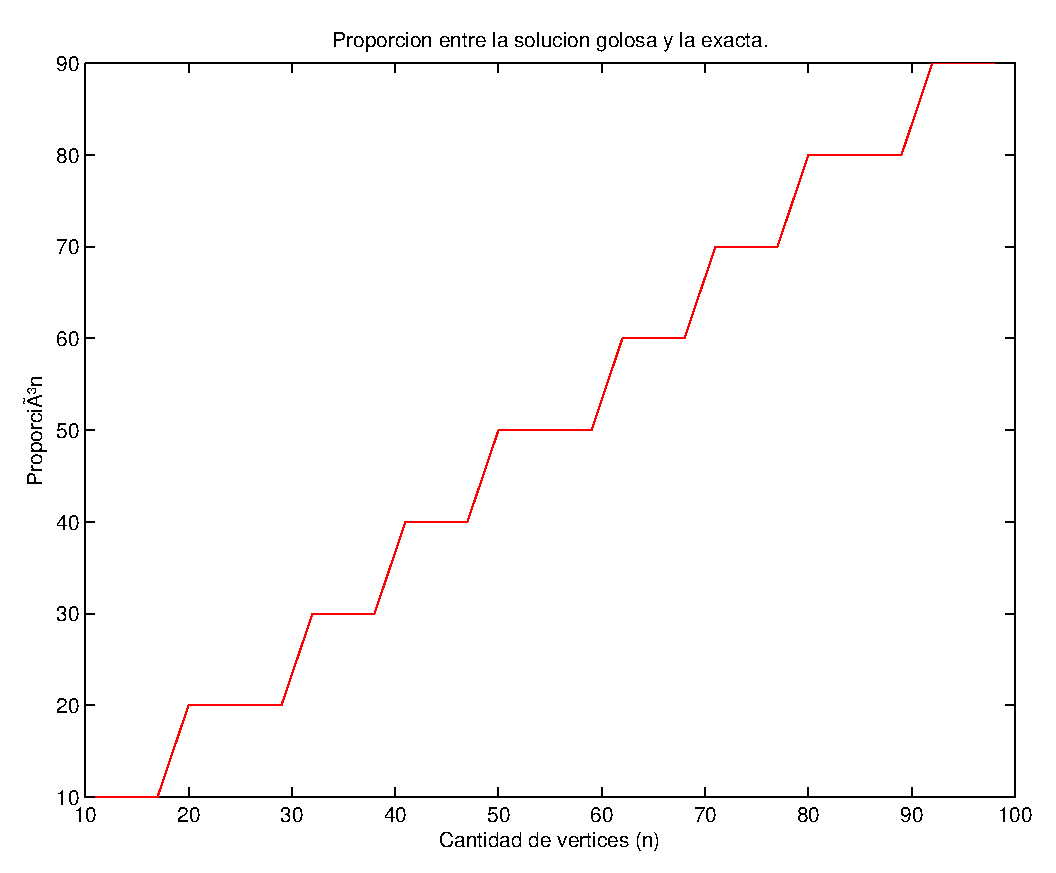
\includegraphics[width=\linewidth]{graficos/goloso_proporcion2.eps}
    \caption{Comparación goloso exacto escalonado}\label{fig:goloso-escalonado}
  \end{minipage}
\end{figure}

En el gráfico \ref{fig:goloso-n2} colocamos la diferencia de $n^2$ para cada $n$, mientras que en el gráfico \ref{fig:goloso-escalonado} utilizamos la siguiente función:
\begin{verbatim}
error(n) = n - (n mod 10)
\end{verbatim}

Cabe aclarar que el segundo gráfico utiliza $n$ mayores a 10, ya que el error tiene que ser mayor o igual a uno. En el caso en que se use un error menor a 1, el algoritmo no funciona ya que esto significaría que es ``más exacto'' que el exacto.

De esta forma, podemos asegurar que nuestro algoritmo goloso no es $\alpha$-aproximado para esta familia de grafos. Esto se puede observar fácilmente, ya que dado un $\alpha$ podemos generar un grafo donde el error proporcional sea mayor a $\alpha$.